\documentclass[12pt]{article}
%Fall 2022
% Some basic packages
\usepackage{standalone}[subpreambles=true]
\usepackage[utf8]{inputenc}
\usepackage[T1]{fontenc}
\usepackage{textcomp}
\usepackage[english]{babel}
\usepackage{url}
\usepackage{graphicx}
%\usepackage{quiver}
\usepackage{float}
\usepackage{enumitem}
\usepackage{lmodern}
\usepackage{comment}
\usepackage{hyperref}
\usepackage[usenames,svgnames,dvipsnames]{xcolor}
\usepackage[margin=1in]{geometry}
\usepackage{pdfpages}

\pdfminorversion=7

% Don't indent paragraphs, leave some space between them
\usepackage{parskip}

% Hide page number when page is empty
\usepackage{emptypage}
\usepackage{subcaption}
\usepackage{multicol}
\usepackage[b]{esvect}

% Math stuff
\usepackage{amsmath, amsfonts, mathtools, amsthm, amssymb}
\usepackage{bbm}
\usepackage{stmaryrd}
\allowdisplaybreaks

% Fancy script capitals
\usepackage{mathrsfs}
\usepackage{cancel}
% Bold math
\usepackage{bm}
% Some shortcuts
\newcommand{\rr}{\ensuremath{\mathbb{R}}}
\newcommand{\zz}{\ensuremath{\mathbb{Z}}}
\newcommand{\qq}{\ensuremath{\mathbb{Q}}}
\newcommand{\nn}{\ensuremath{\mathbb{N}}}
\newcommand{\ff}{\ensuremath{\mathbb{F}}}
\newcommand{\cc}{\ensuremath{\mathbb{C}}}
\newcommand{\ee}{\ensuremath{\mathbb{E}}}
\newcommand{\hh}{\ensuremath{\mathbb{H}}}
\renewcommand\O{\ensuremath{\emptyset}}
\newcommand{\norm}[1]{{\left\lVert{#1}\right\rVert}}
\newcommand{\dbracket}[1]{{\left\llbracket{#1}\right\rrbracket}}
\newcommand{\ve}[1]{{\bm{#1}}}
\newcommand\allbold[1]{{\boldmath\textbf{#1}}}
\DeclareMathOperator{\lcm}{lcm}
\DeclareMathOperator{\im}{im}
\DeclareMathOperator{\coim}{coim}
\DeclareMathOperator{\dom}{dom}
\DeclareMathOperator{\tr}{tr}
\DeclareMathOperator{\rank}{rank}
\DeclareMathOperator*{\var}{Var}
\DeclareMathOperator*{\ev}{E}
\DeclareMathOperator{\dg}{deg}
\DeclareMathOperator{\aff}{aff}
\DeclareMathOperator{\conv}{conv}
\DeclareMathOperator{\inte}{int}
\DeclareMathOperator*{\argmin}{argmin}
\DeclareMathOperator*{\argmax}{argmax}
\DeclareMathOperator{\graph}{graph}
\DeclareMathOperator{\sgn}{sgn}
\DeclareMathOperator*{\Rep}{Rep}
\DeclareMathOperator{\Proj}{Proj}
\DeclareMathOperator{\mat}{mat}
\DeclareMathOperator{\diag}{diag}
\DeclareMathOperator{\aut}{Aut}
\DeclareMathOperator{\gal}{Gal}
\DeclareMathOperator{\inn}{Inn}
\DeclareMathOperator{\edm}{End}
\DeclareMathOperator{\Hom}{Hom}
\DeclareMathOperator{\ext}{Ext}
\DeclareMathOperator{\tor}{Tor}
\DeclareMathOperator{\Span}{Span}
\DeclareMathOperator{\Stab}{Stab}
\DeclareMathOperator{\cont}{cont}
\DeclareMathOperator{\Ann}{Ann}
\DeclareMathOperator{\Div}{div}
\DeclareMathOperator{\curl}{curl}
\DeclareMathOperator{\nat}{Nat}
\DeclareMathOperator{\gr}{Gr}
\DeclareMathOperator{\vect}{Vect}
\DeclareMathOperator{\id}{id}
\DeclareMathOperator{\Mod}{Mod}
\DeclareMathOperator{\sign}{sign}
\DeclareMathOperator{\Surf}{Surf}
\DeclareMathOperator{\fcone}{fcone}
\DeclareMathOperator{\Rot}{Rot}
\DeclareMathOperator{\grad}{grad}
\DeclareMathOperator{\atan2}{atan2}
\DeclareMathOperator{\Ric}{Ric}
\let\vec\relax
\DeclareMathOperator{\vec}{vec}
\let\Re\relax
\DeclareMathOperator{\Re}{Re}
\let\Im\relax
\DeclareMathOperator{\Im}{Im}
% Put x \to \infty below \lim
\let\svlim\lim\def\lim{\svlim\limits}

%wide hat
\usepackage{scalerel,stackengine}
\stackMath
\newcommand*\wh[1]{%
\savestack{\tmpbox}{\stretchto{%
  \scaleto{%
    \scalerel*[\widthof{\ensuremath{#1}}]{\kern-.6pt\bigwedge\kern-.6pt}%
    {\rule[-\textheight/2]{1ex}{\textheight}}%WIDTH-LIMITED BIG WEDGE
  }{\textheight}% 
}{0.5ex}}%
\stackon[1pt]{#1}{\tmpbox}%
}
\parskip 1ex

%Make implies and impliedby shorter
\let\implies\Rightarrow
\let\impliedby\Leftarrow
\let\iff\Leftrightarrow
\let\epsilon\varepsilon

% Add \contra symbol to denote contradiction
\usepackage{stmaryrd} % for \lightning
\newcommand\contra{\scalebox{1.5}{$\lightning$}}

% \let\phi\varphi

% Command for short corrections
% Usage: 1+1=\correct{3}{2}

\definecolor{correct}{HTML}{009900}
\newcommand\correct[2]{\ensuremath{\:}{\color{red}{#1}}\ensuremath{\to }{\color{correct}{#2}}\ensuremath{\:}}
\newcommand\green[1]{{\color{correct}{#1}}}

% horizontal rule
\newcommand\hr{
    \noindent\rule[0.5ex]{\linewidth}{0.5pt}
}

% hide parts
\newcommand\hide[1]{}

% si unitx
\usepackage{siunitx}
\sisetup{locale = FR}

%allows pmatrix to stretch
\makeatletter
\renewcommand*\env@matrix[1][\arraystretch]{%
  \edef\arraystretch{#1}%
  \hskip -\arraycolsep
  \let\@ifnextchar\new@ifnextchar
  \array{*\c@MaxMatrixCols c}}
\makeatother

\renewcommand{\arraystretch}{0.8}

\renewcommand{\baselinestretch}{1.5}

\usepackage{graphics}
\usepackage{epstopdf}

\RequirePackage{hyperref}
%%
%% Add support for color in order to color the hyperlinks.
%% 
\hypersetup{
  colorlinks = true,
  urlcolor = blue,
  citecolor = blue
}
%%fakesection Links
\hypersetup{
    colorlinks,
    linkcolor={red!50!black},
    citecolor={green!50!black},
    urlcolor={blue!80!black}
}
%customization of cleveref
\RequirePackage[capitalize,nameinlink]{cleveref}[0.19]

% Per SIAM Style Manual, "section" should be lowercase
\crefname{section}{section}{sections}
\crefname{subsection}{subsection}{subsections}
\Crefname{section}{Section}{Sections}
\Crefname{subsection}{Subsection}{Subsections}

% Per SIAM Style Manual, "Figure" should be spelled out in references
\Crefname{figure}{Figure}{Figures}

% Per SIAM Style Manual, don't say equation in front on an equation.
\crefformat{equation}{\textup{#2(#1)#3}}
\crefrangeformat{equation}{\textup{#3(#1)#4--#5(#2)#6}}
\crefmultiformat{equation}{\textup{#2(#1)#3}}{ and \textup{#2(#1)#3}}
{, \textup{#2(#1)#3}}{, and \textup{#2(#1)#3}}
\crefrangemultiformat{equation}{\textup{#3(#1)#4--#5(#2)#6}}%
{ and \textup{#3(#1)#4--#5(#2)#6}}{, \textup{#3(#1)#4--#5(#2)#6}}{, and \textup{#3(#1)#4--#5(#2)#6}}

% But spell it out at the beginning of a sentence.
\Crefformat{equation}{#2Equation~\textup{(#1)}#3}
\Crefrangeformat{equation}{Equations~\textup{#3(#1)#4--#5(#2)#6}}
\Crefmultiformat{equation}{Equations~\textup{#2(#1)#3}}{ and \textup{#2(#1)#3}}
{, \textup{#2(#1)#3}}{, and \textup{#2(#1)#3}}
\Crefrangemultiformat{equation}{Equations~\textup{#3(#1)#4--#5(#2)#6}}%
{ and \textup{#3(#1)#4--#5(#2)#6}}{, \textup{#3(#1)#4--#5(#2)#6}}{, and \textup{#3(#1)#4--#5(#2)#6}}

% Make number non-italic in any environment.
\crefdefaultlabelformat{#2\textup{#1}#3}

% Environments
\makeatother
% For box around Definition, Theorem, \ldots
%%fakesection Theorems
\usepackage{thmtools}
\usepackage[framemethod=TikZ]{mdframed}

\theoremstyle{definition}
\mdfdefinestyle{mdbluebox}{%
	roundcorner = 10pt,
	linewidth=1pt,
	skipabove=12pt,
	innerbottommargin=9pt,
	skipbelow=2pt,
	nobreak=true,
	linecolor=blue,
	backgroundcolor=TealBlue!5,
}
\declaretheoremstyle[
	headfont=\sffamily\bfseries\color{MidnightBlue},
	mdframed={style=mdbluebox},
	headpunct={\\[3pt]},
	postheadspace={0pt}
]{thmbluebox}

\mdfdefinestyle{mdredbox}{%
	linewidth=0.5pt,
	skipabove=12pt,
	frametitleaboveskip=5pt,
	frametitlebelowskip=0pt,
	skipbelow=2pt,
	frametitlefont=\bfseries,
	innertopmargin=4pt,
	innerbottommargin=8pt,
	nobreak=false,
	linecolor=RawSienna,
	backgroundcolor=Salmon!5,
}
\declaretheoremstyle[
	headfont=\bfseries\color{RawSienna},
	mdframed={style=mdredbox},
	headpunct={\\[3pt]},
	postheadspace={0pt},
]{thmredbox}

\declaretheorem[%
style=thmbluebox,name=Theorem,numberwithin=section]{thm}
\declaretheorem[style=thmbluebox,name=Lemma,sibling=thm]{lem}
\declaretheorem[style=thmbluebox,name=Proposition,sibling=thm]{prop}
\declaretheorem[style=thmbluebox,name=Corollary,sibling=thm]{coro}
\declaretheorem[style=thmredbox,name=Example,sibling=thm]{eg}

\mdfdefinestyle{mdgreenbox}{%
	roundcorner = 10pt,
	linewidth=1pt,
	skipabove=12pt,
	innerbottommargin=9pt,
	skipbelow=2pt,
	nobreak=true,
	linecolor=ForestGreen,
	backgroundcolor=ForestGreen!5,
}

\declaretheoremstyle[
	headfont=\bfseries\sffamily\color{ForestGreen!70!black},
	bodyfont=\normalfont,
	spaceabove=2pt,
	spacebelow=1pt,
	mdframed={style=mdgreenbox},
	headpunct={ --- },
]{thmgreenbox}

\declaretheorem[style=thmgreenbox,name=Definition,sibling=thm]{defn}

\mdfdefinestyle{mdgreenboxsq}{%
	linewidth=1pt,
	skipabove=12pt,
	innerbottommargin=9pt,
	skipbelow=2pt,
	nobreak=true,
	linecolor=ForestGreen,
	backgroundcolor=ForestGreen!5,
}
\declaretheoremstyle[
	headfont=\bfseries\sffamily\color{ForestGreen!70!black},
	bodyfont=\normalfont,
	spaceabove=2pt,
	spacebelow=1pt,
	mdframed={style=mdgreenboxsq},
	headpunct={},
]{thmgreenboxsq}
\declaretheoremstyle[
	headfont=\bfseries\sffamily\color{ForestGreen!70!black},
	bodyfont=\normalfont,
	spaceabove=2pt,
	spacebelow=1pt,
	mdframed={style=mdgreenboxsq},
	headpunct={},
]{thmgreenboxsq*}

\mdfdefinestyle{mdblackbox}{%
	skipabove=8pt,
	linewidth=3pt,
	rightline=false,
	leftline=true,
	topline=false,
	bottomline=false,
	linecolor=black,
	backgroundcolor=RedViolet!5!gray!5,
}
\declaretheoremstyle[
	headfont=\bfseries,
	bodyfont=\normalfont\small,
	spaceabove=0pt,
	spacebelow=0pt,
	mdframed={style=mdblackbox}
]{thmblackbox}

\theoremstyle{plain}
\declaretheorem[name=Question,sibling=thm,style=thmblackbox]{ques}
\declaretheorem[name=Remark,sibling=thm,style=thmgreenboxsq]{remark}
\declaretheorem[name=Remark,sibling=thm,style=thmgreenboxsq*]{remark*}
\newtheorem{ass}[thm]{Assumptions}

\theoremstyle{definition}
\newtheorem*{problem}{Problem}
\newtheorem{claim}[thm]{Claim}
\theoremstyle{remark}
\newtheorem*{case}{Case}
\newtheorem*{notation}{Notation}
\newtheorem*{note}{Note}
\newtheorem*{motivation}{Motivation}
\newtheorem*{intuition}{Intuition}
\newtheorem*{conjecture}{Conjecture}

% Make section starts with 1 for report type
%\renewcommand\thesection{\arabic{section}}

% End example and intermezzo environments with a small diamond (just like proof
% environments end with a small square)
\usepackage{etoolbox}
\AtEndEnvironment{vb}{\null\hfill$\diamond$}%
\AtEndEnvironment{intermezzo}{\null\hfill$\diamond$}%
% \AtEndEnvironment{opmerking}{\null\hfill$\diamond$}%

% Fix some spacing
% http://tex.stackexchange.com/questions/22119/how-can-i-change-the-spacing-before-theorems-with-amsthm
\makeatletter
\def\thm@space@setup{%
  \thm@preskip=\parskip \thm@postskip=0pt
}

% Fix some stuff
% %http://tex.stackexchange.com/questions/76273/multiple-pdfs-with-page-group-included-in-a-single-page-warning
\pdfsuppresswarningpagegroup=1


% My name
\author{Jaden Wang}



\begin{document}
\centerline {\textsf{\textbf{\LARGE{Homework 1}}}}
\centerline {Jaden Wang}
\vspace{.15in}
\begin{problem}[1]
$ (\implies)$: suppose $ \gamma: I \to X$ is a path between $ x$ and  $ y$. Let $ p: \{*\} \times I \to I, (*,t) \mapsto t$ be the canonical identification (and projection and thus continuous). We see that $ \gamma \circ p(*,0) = e_x(*)$ and $ \gamma \circ p(*,1) = e_y(*)$. As composition of continuous functions are continuous, $ \gamma \circ p$ is a homotopy between $ e_x$ and  $ e_y$.

 $ (\impliedby):$ suppose $ e_x \simeq e_y$, \emph{i.e.} there exists a homotopy $ H: \{*\} \times I \to X$ s.t.\ $ H(*,0) = e_x(*) = x$ and  $ H(*,1) = e_y(*) = y$. Then let $i: I \to \{*\} \times I , t \mapsto (*,t)$ be the canonical inclusion which is continuous. Then $ H \circ i: I \to X$ is clearly a path between $ x$ and  $ y$.
\end{problem}
\begin{problem}[2]
$ 1 \implies 2:$ suppose $ X$ is contractible,  \emph{i.e.} $ \text{id}_{ X} \simeq e_{x_0}$ via a homotopy $ H$. Then given a map $ f: X \to Y$, we see that
\begin{align*}
	f= f \circ \text{id}_{ X} \simeq f \circ e_{x_0} = e_{f(x_0)}
\end{align*}
via a homotopy $ f \circ H$.

$ 2 \implies 3:$ suppose for a given space $ X$, every map $ f:X \to Y$ is null-homotopic for any $ Y$. In particular, $ \text{id}_{ X} \simeq e_{x_0}$ via a homotopy $ H$ when we let $ Y=X$. Then for any $ Y$ and a map $ f: Y \to X$, let $ x_0$ be any point in $ f(Y)$ and we see that
\begin{align*}
	f= \text{id}_{ X} \circ f \simeq e_{x_0} \circ f = e'_{x_0},
\end{align*}
where $ e'_{x_0}: Y \to X, y \mapsto x_0$, via the homotopy $ H': Y \times I \to X, (y,t) \mapsto H(f(y),t)$.

$ 3 \implies 1:$ this is immediate by letting $ Y = X$ and considering  $ \text{id}_{ X}$, just like above.
\end{problem}

\begin{problem}[4]
	We wish to exhibit a homeomorphism. Consider $ S^{n}$ for any $ n$ to be the unit sphere of $ \rr^{n+1}$. Define $ \phi: S^{m} * S^{n} \to S^{m+n+1} \subseteq \rr^{m+n+2}, [(x,t,y)] \mapsto \cos \left( \frac{t \pi}{2} \right) (x,0) + \sin \left( \frac{t \pi}{ 2} \right) (0,y)$. It is easy to verify that the image indeed has unit norm. The map is well-defined: at $ t=0$, the  $ y$-component vanishes so  $ \phi([(x,t,y_1)]) = \phi[(x,t,y_2)] = (x,0)$; $ t=1$ is similar, and that's all the nontrivial equivalence classes we need to check. The map is clearly continuous because projection and trig functions are continuous, and so are their compositions (with invoking universal property of quotient map). It is also a bijection. Given any  $ (a,b) \in S^{m+n+1}$, where $ a \in \rr^{m+1}$ and $ b \in \rr^{n+1}$, $ (a,b)$ is in one of the ``quadrant" of $ S^{m+n+1}$. Let $ x = \frac{a}{ \norm{ a} }$ or 0 if $ a=0$, $y = \frac{b}{ \norm{ b} }$ or 0 if $ b=0$, and $ t =\frac{2}{ \pi} \arctan \left( \frac{\norm{ b} }{\norm{ a} } \right) \in [0,1)$ (since we stay in a quadrant) or 1 if $ a=0$. Then the map $ (a,b) \mapsto [(x,t,y)]$ is $ \phi^{-1}$:
\begin{align*}
	\phi ^{-1} \circ \phi([x,t,y]) &= \phi ^{-1} \left( \cos \left( \frac{t \pi}{ 2} \right)x, \sin \left( \frac{t \pi}{ 2} \right) y \right)  \\
				       &=\begin{cases}
					       [x,t,y] & t \neq 0,1 \text{ or } x,y \neq 0 \\
					       [x,0,0] & t = 0 \text{ or }y=0 \\
					       [0,1,y] & t = 1 \text{ or } x=0 \\
				       \end{cases}\\
				       &= [x,t,y] 
\end{align*}
It is easy to verify the other direction. Thus, we have shown that $ \phi$ is a well-defined bijective continuous map. Since $ S^{m} * S^{n}$ is a quotient of the compact space $ S^{m} \times I \times S^{n}$ and therefore also compact, and $ S^{m+n+1}$ is Hausdorff, it follows that $ \phi$ is a homeomorphism as desired.
~\begin{figure}[H]
	\centering
	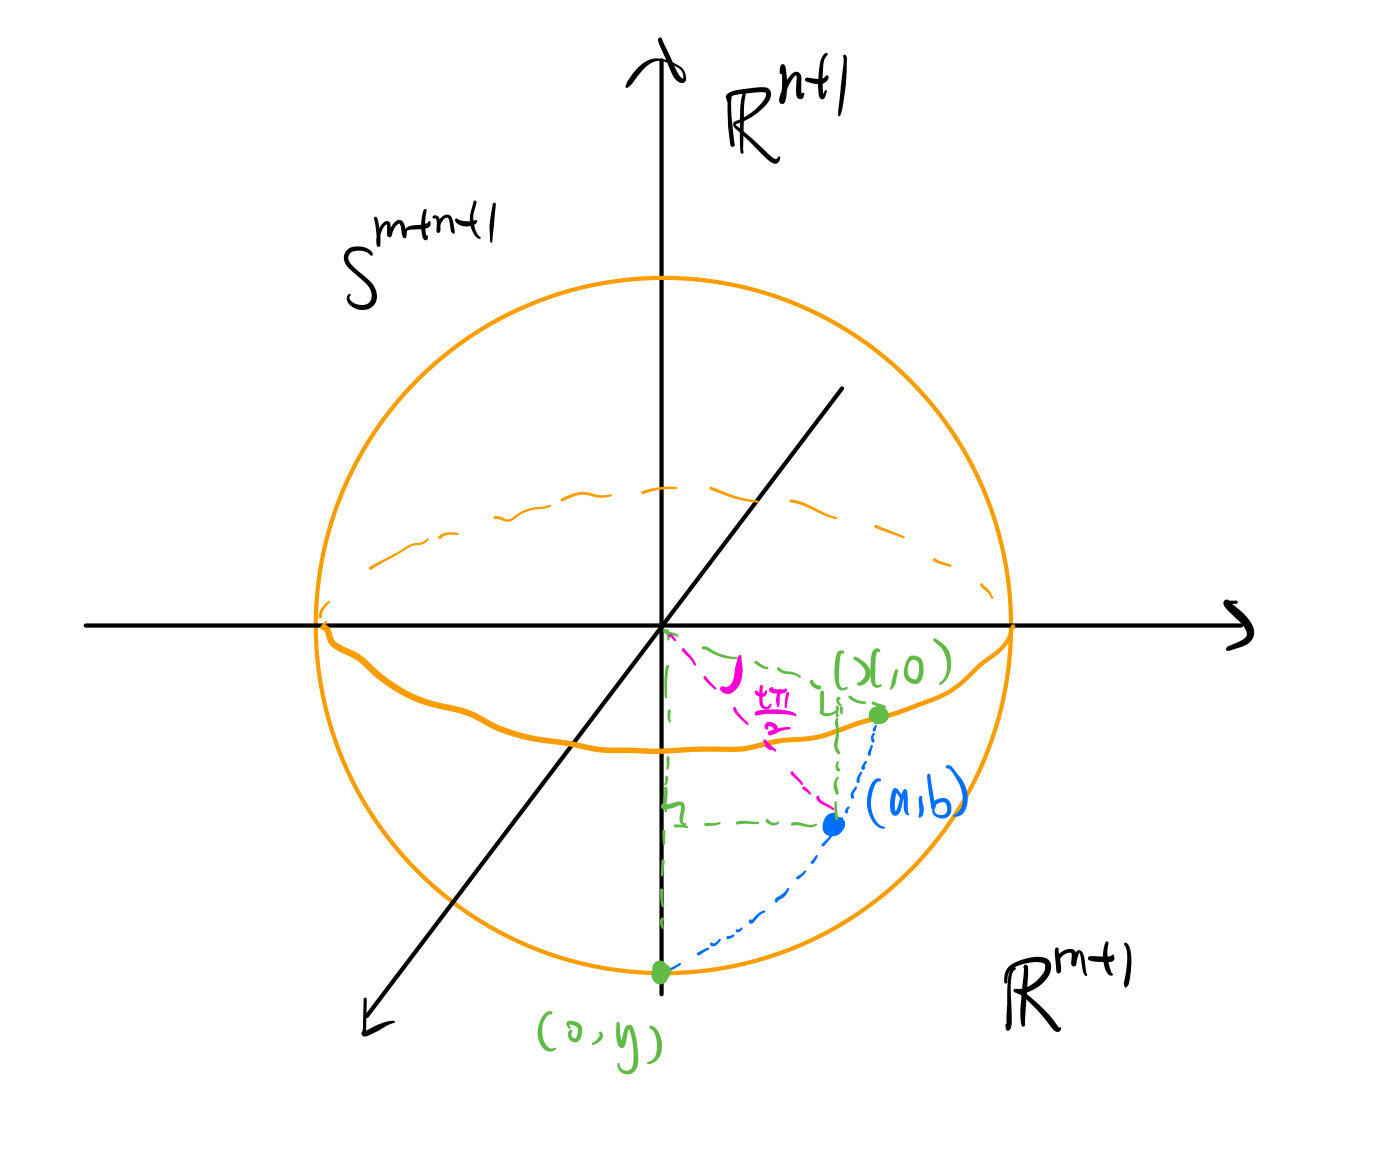
\includegraphics[width=0.6\textwidth]{./figures/join.png}
	\caption{Visualizing $ \phi ^{-1}$.}
\end{figure}
\end{problem}
\begin{problem}[5]
For every $ n$, we see that the $ n$-skeleton is constructed by gluing two $ n$-cells, denoted  $ D_1^{n}$ and $D_2^{n}$, via characteristic maps $ \Phi_1^{n}$ and $ \Phi_2^{n}$. Then each $ n$-skeleton yields three $ n$-subcomplexes: $ \Phi_1^{n}(D_1^{n})$, $ \Phi_2^{n}(D_2^{n})$, and $ (S^{\infty})^{(n)}$. Enumerating over all $ n \in \nn$ gives all the subcomplexes of $ S^{\infty}$.
\end{problem}
\begin{problem}[7]
For $ X \times Y$, we start with $ 0$-skeleton $ (X \times Y)^{(0)}$ as a collection of discrete points. Then inductively assuming we have the $ (n-1)$-skeleton  $ (X \times Y)^{(n-1)}$, we obtain an $ n$-cell $ D_{ \alpha}^{m} \times D_{ \beta}^{k}$ of $ X \times Y$ where $ D_{ \alpha}^{m}$ and $ D_{ \beta}^{n}$ are $ m$-cell and $ k$-cell of $ X$ and  $ Y$, respectively, and $ n=m+k$. Each of these $ n$-cell is glued to $ (X \times Y)^{(n-1)}$ via the attaching map $ \theta_{ \alpha \beta}$ constructed as follows:

Let $ \phi_{ \alpha}: \partial D_{ \alpha}^{m} \to X^{(m-1)}$ and $ \psi_{ \beta}: \partial D_{ \beta}^{k} \to Y^{k-1}$ be the attaching maps, and $ \Phi_{ \alpha}$ and $ \Psi_{ \beta}$ be the corresponding characteristic maps. We see that the boundary of the $ n$-cell $ \partial (D_{ \alpha}^{m} \times D_{ \beta}^{k}) = ( \partial D_{ \alpha}^{m} \times D_{ \beta}^{k}) \cup (D_{ \alpha}^{m} \times \partial D_{ \beta}^{k})$, and we naturally obtain an attaching map on this domain as follows:
\begin{align*}
\theta_{ \alpha \beta} (x,y):= \begin{cases}	
	(\phi_{ \alpha}(x), \Psi_{ \beta}(y)) & x \in \partial D_{ \alpha}^{m} \\
	(\Phi_{ \alpha}(x), \psi_{ \beta}(y)) & y \in \partial D_{ \beta} ^{k}\\
\end{cases}
\end{align*}
Since the intersection of the domains of two maps is $ \partial D_{ \alpha}^{m} \times \partial D_{ \beta}^{k}$ which is closed and they agree on the intersection as  $ (\phi_{ \alpha},\psi_{ \beta})$, $ \theta_{ \alpha \beta}$ is continuous by pasting lemma. Iterating over all $ \alpha$ and $ \beta$ this way, the resulting characteristic maps applied to all $ n$-cells of  $ X \times Y$ yield $ (X \times Y)^{(n)}$.

Let $ S^{1}$ be built with a single 0-cell $ p$ and a single 1-cell $ \alpha$, with the attaching map $ \phi^{1}$ be gluing two endpoints of $ \alpha$ to $ p$. Then $ S^{1} \times S^{1}$ has the following CW structure:
\begin{itemize}
	\item 0-cell: $ \{p_1\} \times \{p_2\}$, a single point.
	\item 1-cell: $ \alpha \times \{p_2\} $ and $ \{p_1\} \times \beta$. We obtain a wedge of two circles as the 1-skeleton via the attaching maps $ (\phi_{ \alpha}^{1}, \text{id}_{ p_2}) $ and $ (\text{id}_{ p_1}, \psi_{ \beta}^{1})$. We see that $ \phi_{ \alpha}^{1}$ and $ \psi_{ \beta}^{1}$ simply identify end points of $ \alpha$ and $ \beta$ respectively.
	\item 2-cell: $ \alpha \times \beta$, a square, with boundary $ (\partial \alpha \times \beta) \cup (\alpha\times  \partial \beta) = (\{0,1\} \times \beta ) \cup ( \alpha \times \{0,1\} )$. The attaching map $ \theta_{ \alpha \beta}$ clearly identifies $\{0\} \times \beta \sim \{1\} \times \beta $ and $ \alpha \times \{0\} \sim \alpha \times \{1\} $ respectively via $ \phi_{ \alpha}^{1}$ and $ \psi_{ \beta}^{1}$ ( \emph{i.e.} the opposite sides of the boundary are identified) and applies characteristic maps ( \emph{i.e.} inclusion then quotient) on the identified $ \alpha$ and $ \beta$.
\end{itemize}
~\begin{figure}[H]
	\centering
	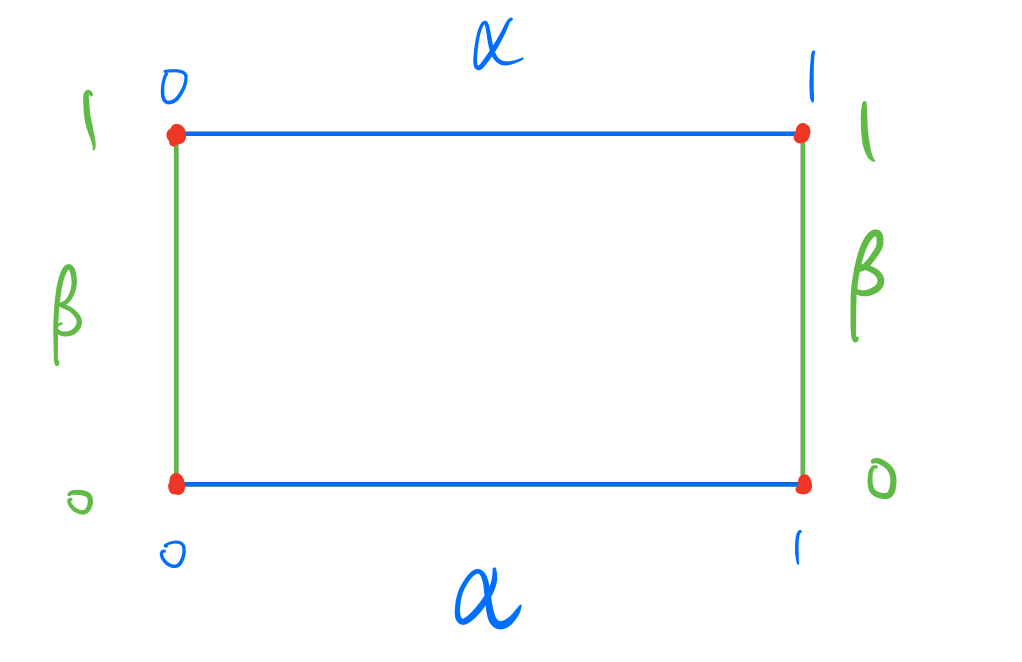
\includegraphics[width=0.4\textwidth]{./figures/torus_cw.png}
	\caption{The attaching map of the 2-cell.}
\end{figure}
\end{problem}

\begin{problem}[8]
	Define a binary opeartion on $ [X,G]$ by pointwise multiplication: given $ [f],[g] \in [X,G]$, $ f \cdot g (x):= f(x) \cdot g(x) \in G$. Let $ f_1,g_1$ be another representative via homotopies $ F,G$, then $ f_1 \cdot g_1 \simeq f \cdot g$ via the homotopy $ H(x,t):= F(x,t)G(x,t)$. Thus the binary operation is well-defined on the equivalence classes and we shall only use the representatives for the rest of the proof. Associativity is inherited from associativity of $ G$. We see that the map $ i: x \mapsto e$ is the identity, since $ (f \cdot i)(x) = f(x) \cdot e = f(x) = e \cdot f(x) = (i \cdot f)(x) $. Finally, given $ f\in [X,G]$, define $ f^{-1}: X \to G, x \mapsto (f(x))^{-1}$. Then clearly $ (f^{-1} \cdot f)(x) = f^{-1}(x) \cdot f(x) = (f(x))^{-1} \cdot f(x) = e = i(x) = f(x) \cdot (f(x))^{-1} = (f \cdot f^{-1})(x)$.

	Given a map $ f: X \to Y$, $ g,h \in [Y,G]$,
\begin{align*}
	(f^* (g \cdot h))(x) &= ((g \cdot h) \circ f)(x) \\
	&= (g \cdot h) (f(x)) \\
	&= (g(f(x)) \cdot h(f(x))) && \text{ pointwise multi} \\
	&= (g \circ f(x)) \cdot (h \circ f(x)) \\
	&= (f^* (g)) (x) \cdot (f^* (h))(x) 
\end{align*}
Thus $ f^* $ is a homomorphism.
\end{problem}
\end{document}
